\chapter{Anhang}
\begin{table}[h]
    \centering
    \caption[Tabelle der Messwerte]{Tabelle der Messwerte.}
    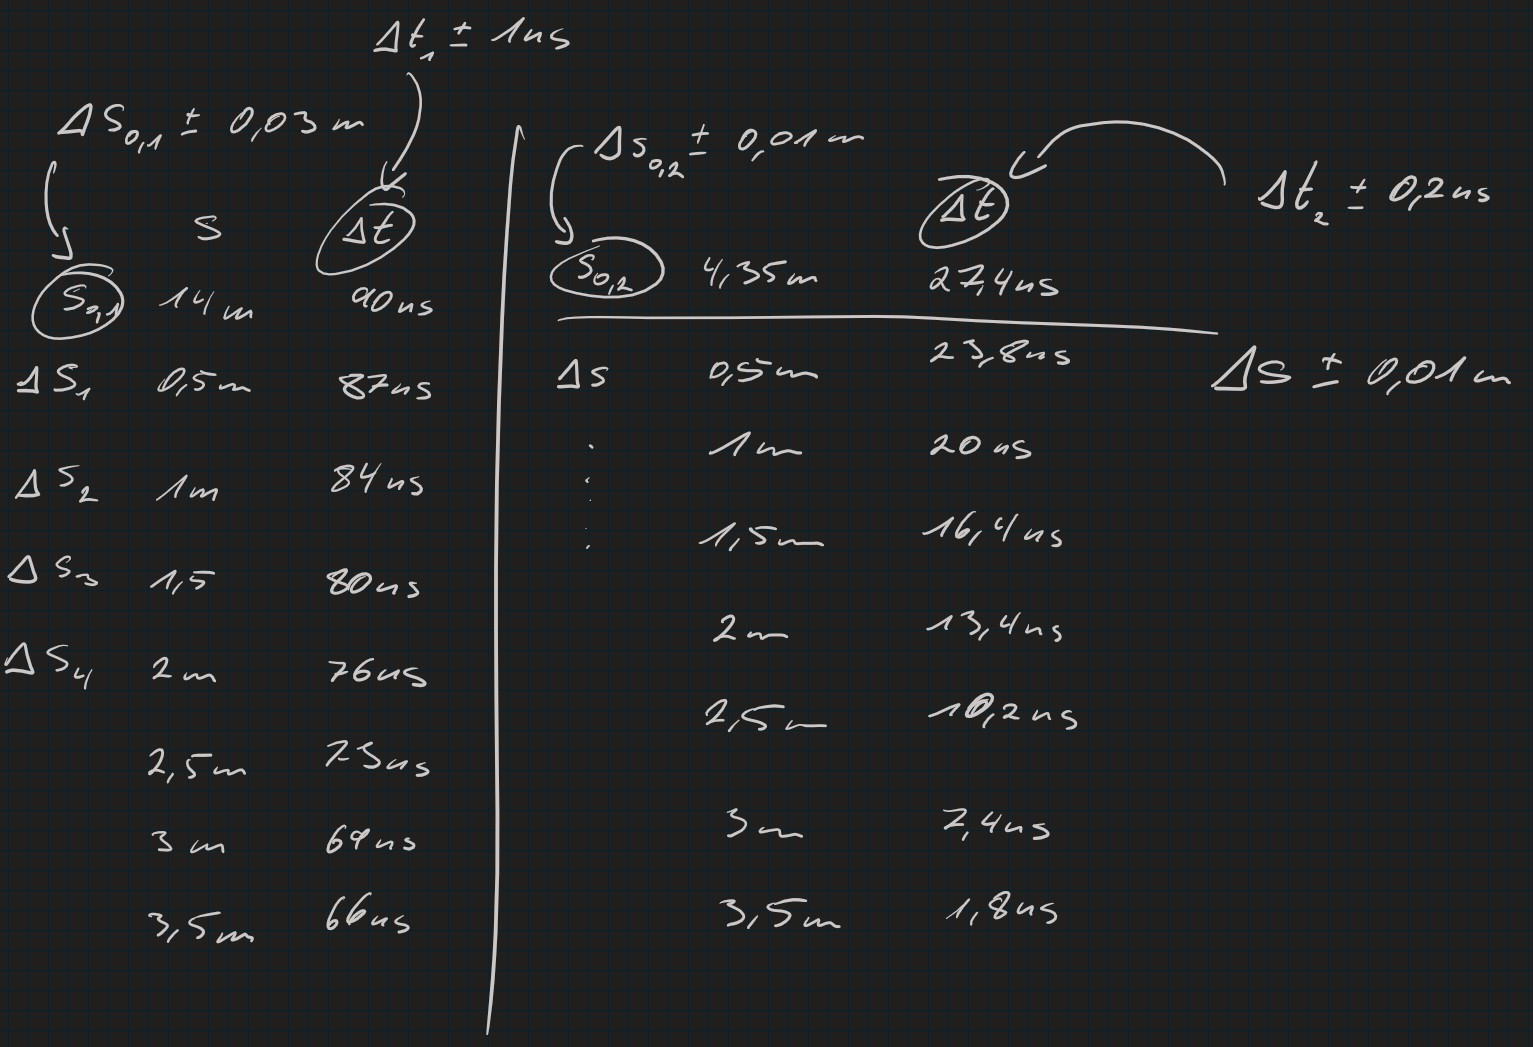
\includegraphics[width=\textwidth]{messungen/tabelle_messwerte.jpg}
    \label{tab:messwerte}
\end{table}
%
\begin{figure}[!ht]
    \centering
    \subfloat[\(\Delta t\)\label{subfig:delta_t}]{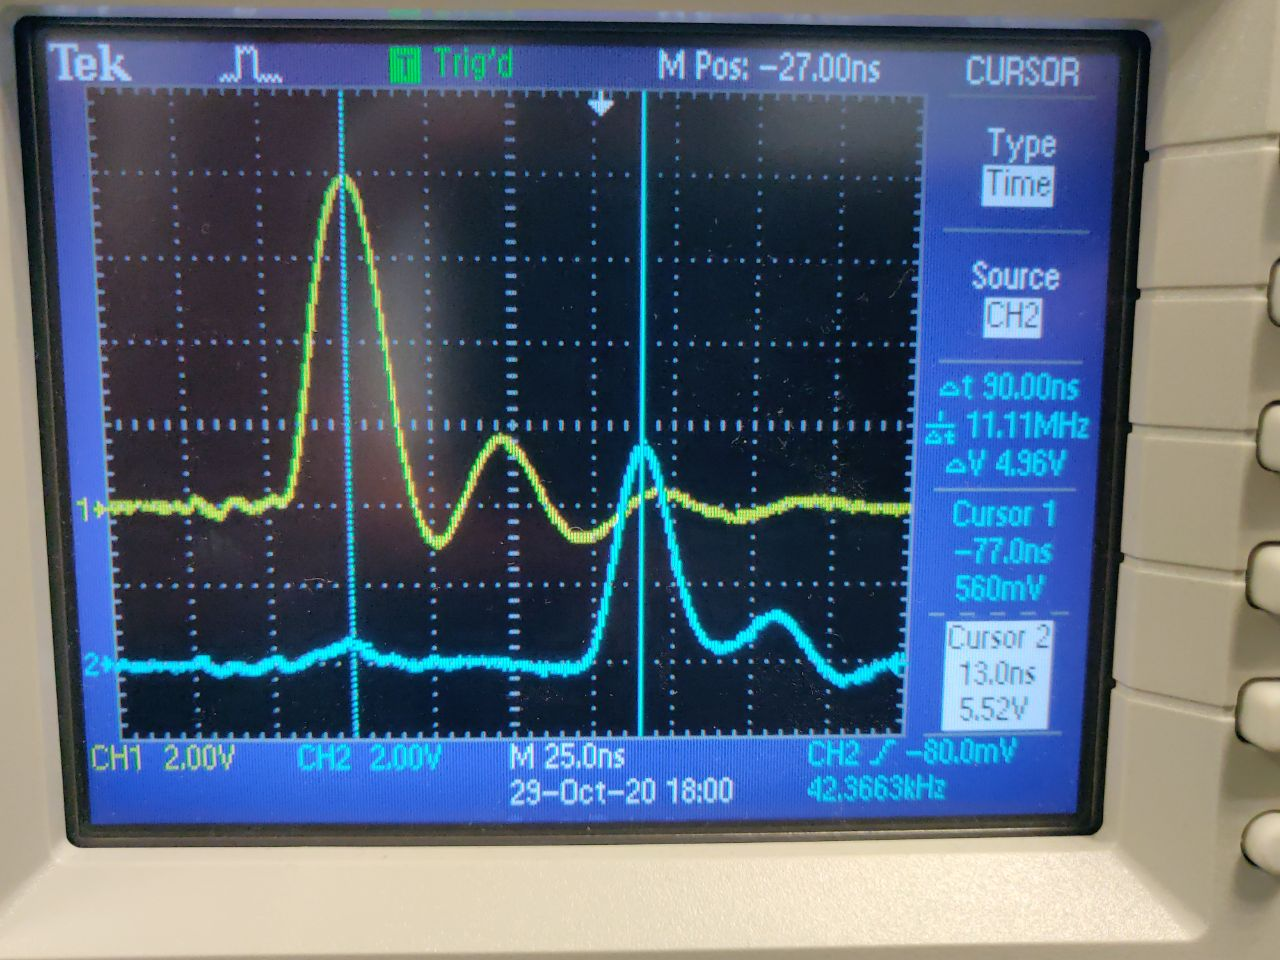
\includegraphics[width=0.45\textwidth]{messungen/delta_t.jpg}}
    \hspace{.05\textwidth}
    \subfloat[\(\hat{U}\)\label{subfig:U_dach}]{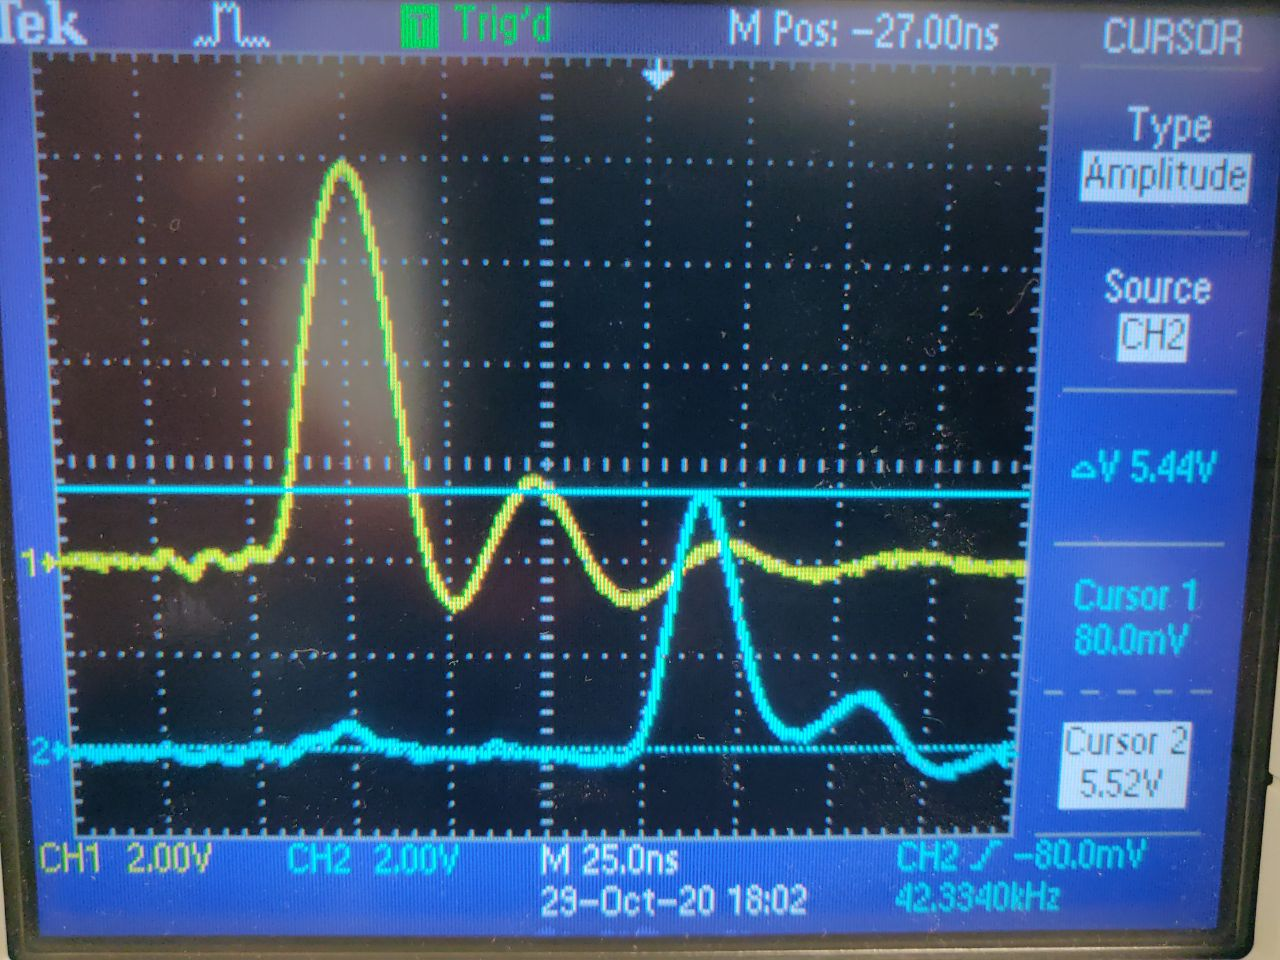
\includegraphics[width=0.45\textwidth]{messungen/U_dach.jpg}}
    \hspace{.2\textwidth}
    \subfloat[\(t_{rise}\)\label{subfig:t_rise}]{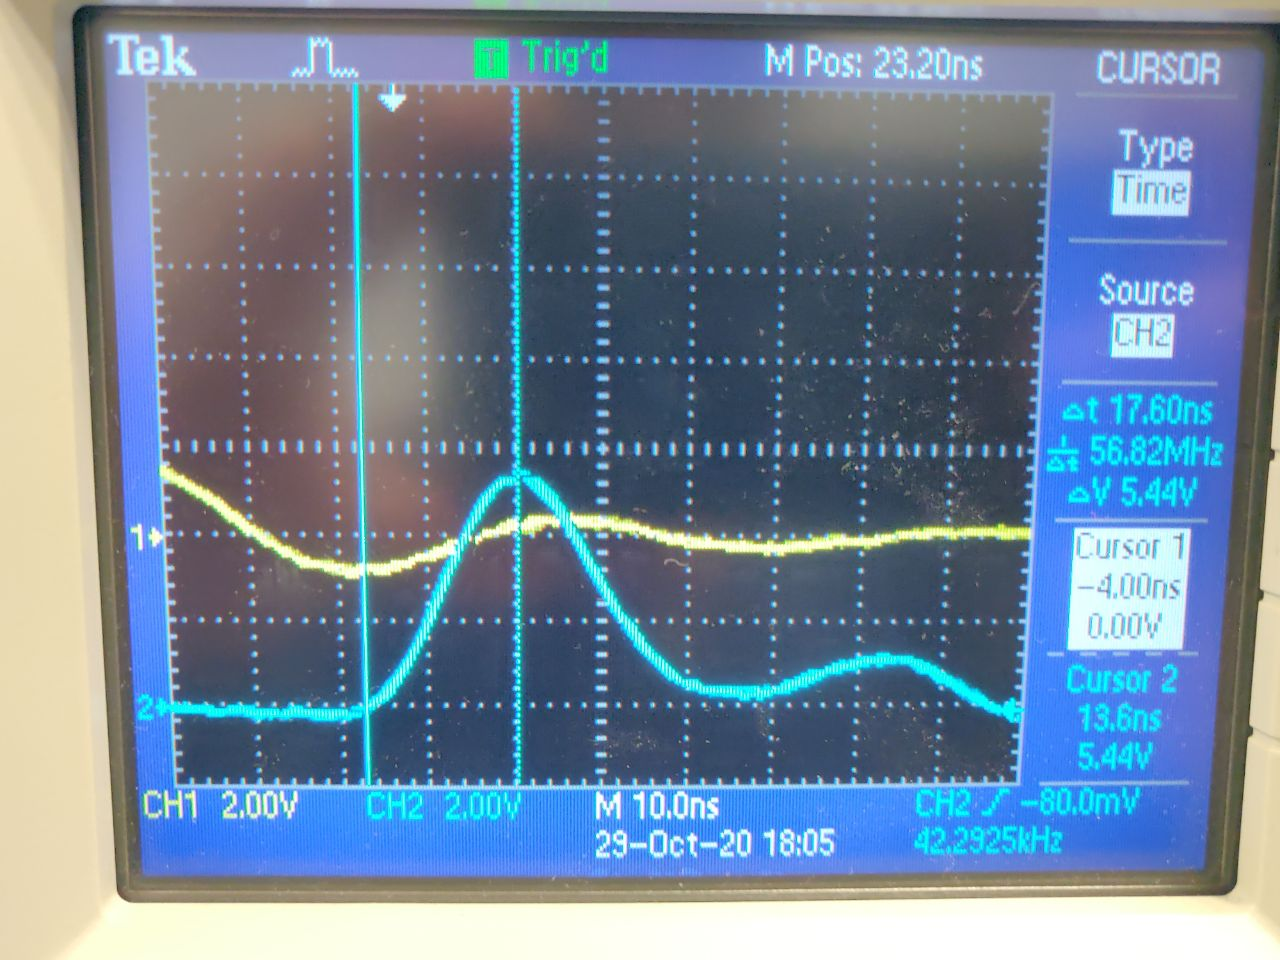
\includegraphics[width=0.45\textwidth]{messungen/t_rise.jpg}}
    \hspace{.05\textwidth}
    \subfloat[\(t_p\)\label{subfig:t_p}]{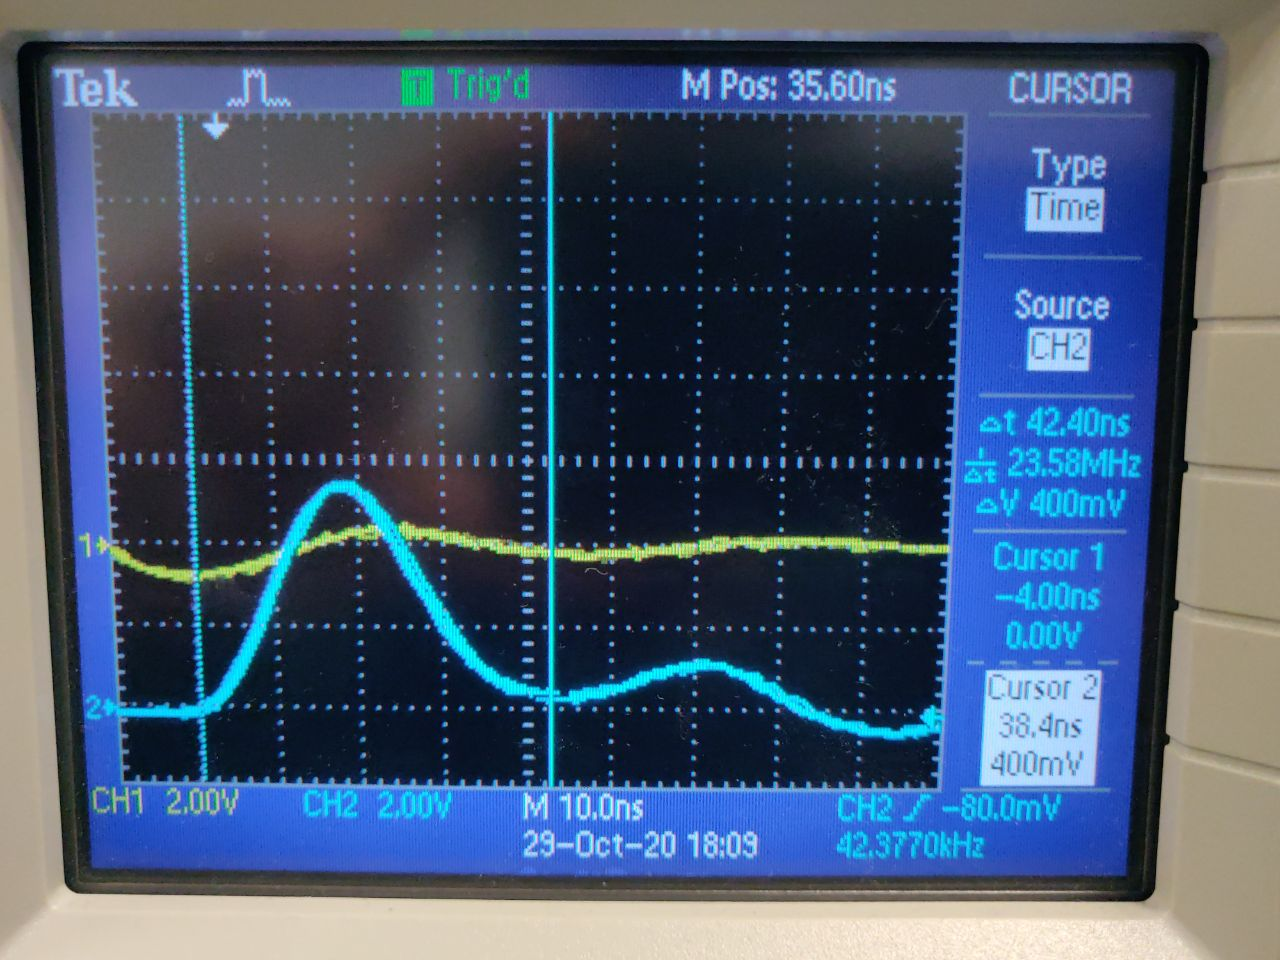
\includegraphics[width=0.45\textwidth]{messungen/t_pulse.jpg}}
    \hspace{.2\textwidth}
    \subfloat[\(f_p\)\label{subfig:f_p}]{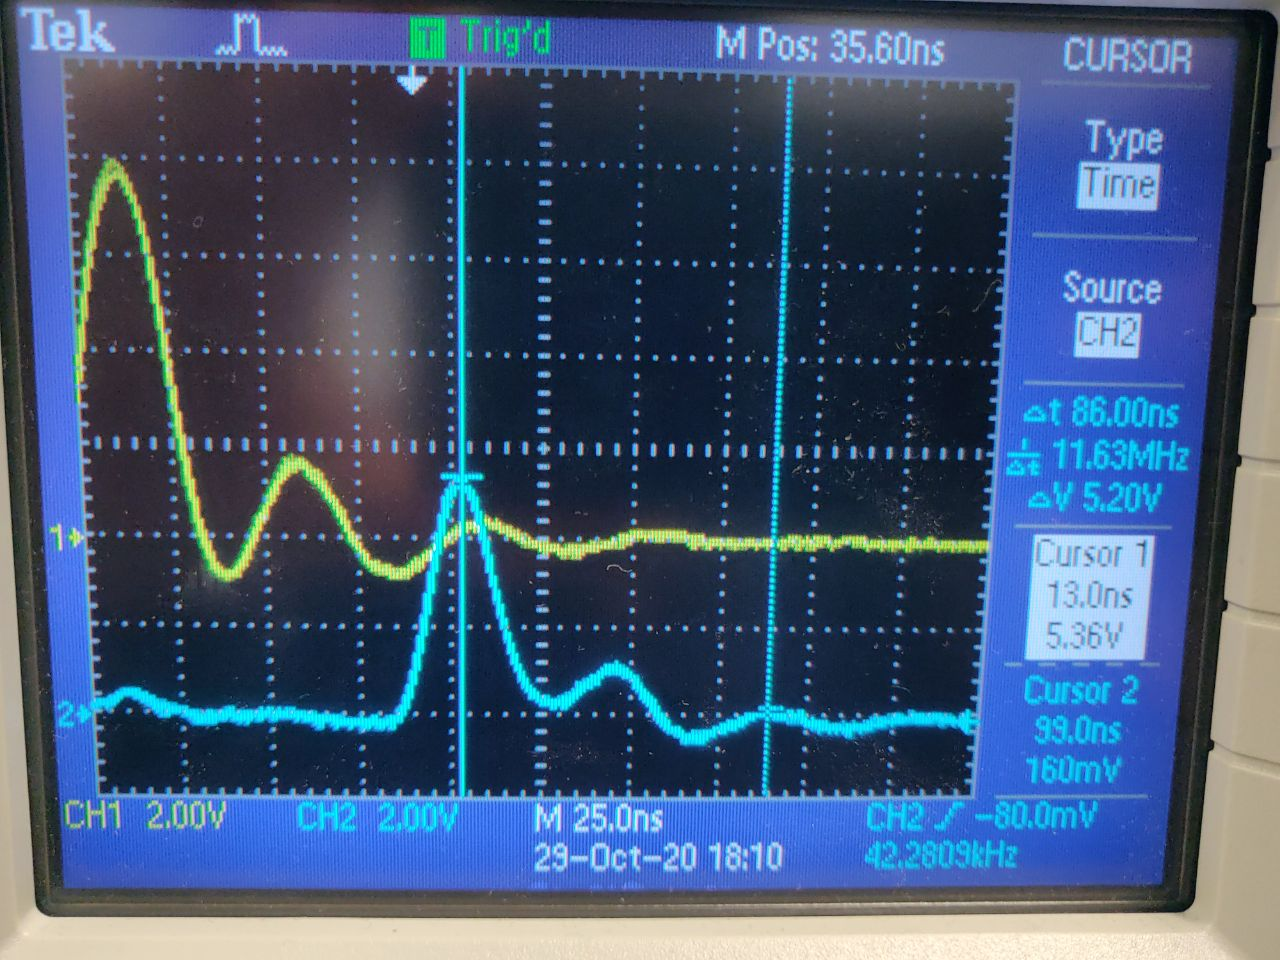
\includegraphics[width=0.45\textwidth]{messungen/freq_schwingung.jpg}}
    \caption[Oszillogramme]{Der Auswertung zu Grunde liegende Oszillogramme.}
 \end{figure}